\documentclass[aspectratio=169,14pt]{beamer}
\usepackage{calc}
\usepackage{graphicx}
\usepackage{fontspec}

\usetheme{Singapore}
\usecolortheme[RGB={41,92,35}]{structure}
\setbeamercolor{section in head/foot}{bg=white}
\setbeamercovered{again covered={\opaqueness<1->{50}}}

\defaultfontfeatures{Mapping=tex-text}
%\setsansfont{Sofia Pro}
\setsansfont{Open Sans}

\title[Advisory Board Meeting]{Overview of beta site}
\subtitle{Advisory Board Meeting}
\institute{Databrary}
\date{April 7, 2014}

\pgfdeclareimage[height=1cm]{databrary}{../databrary}
\logo{\pgfuseimage{databrary}}

\begin{document}

\begin{frame}
	\titlepage
\end{frame}

\section{Progress}

\begin{frame}{6 months ago}{Website}
	\begin{itemize}
		\item	Lots of videos
		\begin{itemize}
			\item Piled up into studies
			\item Minimal organization
		\end{itemize}
		\item	``Static'' views
		\begin{itemize}
			\item Single presentation option
			\item Limited flexibility
		\end{itemize}
	\end{itemize}
\end{frame}

\begin{frame}{Updates}{Website}
	\begin{itemize}
		\item	Revised technical requirements
		\begin{itemize}
			\item Flexible discovery options
			\begin{itemize}
				\item searching: by keyword, text, descriptions, names, etc. (text box)
				\item filtering: limiting results by age, gender, numeric values (side bar)
			\end{itemize}
			\item Efficient, intuitive editing, uploading
			\item High-level visualizations, summaries
			\item API, scripting interface
		\end{itemize}
		\item Built new completely dynamic JS interface, using API
	\end{itemize}
\end{frame}

\begin{frame}{Updates}{Previously collected data}
	\begin{itemize}
		\item Learned a lot from manually curating and organizing existing and new datasets
		\item Broadened types of possible, standard metadata
		\item Developed better ways to group and relate data, studies, datasets
	\end{itemize}
\end{frame}

\begin{frame}{Updates}{Data model}
	\begin{itemize}
		\item There are always exceptions, irregularities in real data
		\begin{itemize}
			\item Missing/multiple videos
			\item Doesn't fit cleanly in defined groups
			\item Excluded and later re-purposed data
			\item Always something \emph{non-rectangular}
		\end{itemize}
		\item Different types of data (classroom, public, longitudinal) have different needs
		\item Need responsive, iterative, ``data-driven'' approach
		\item Better understanding of constraints, required flexibility
	\end{itemize}
\end{frame}

\section{Data structures}

\begin{frame}{Session}{Basic organizational unit}
	\begin{columns}
	\column{2.5in}
	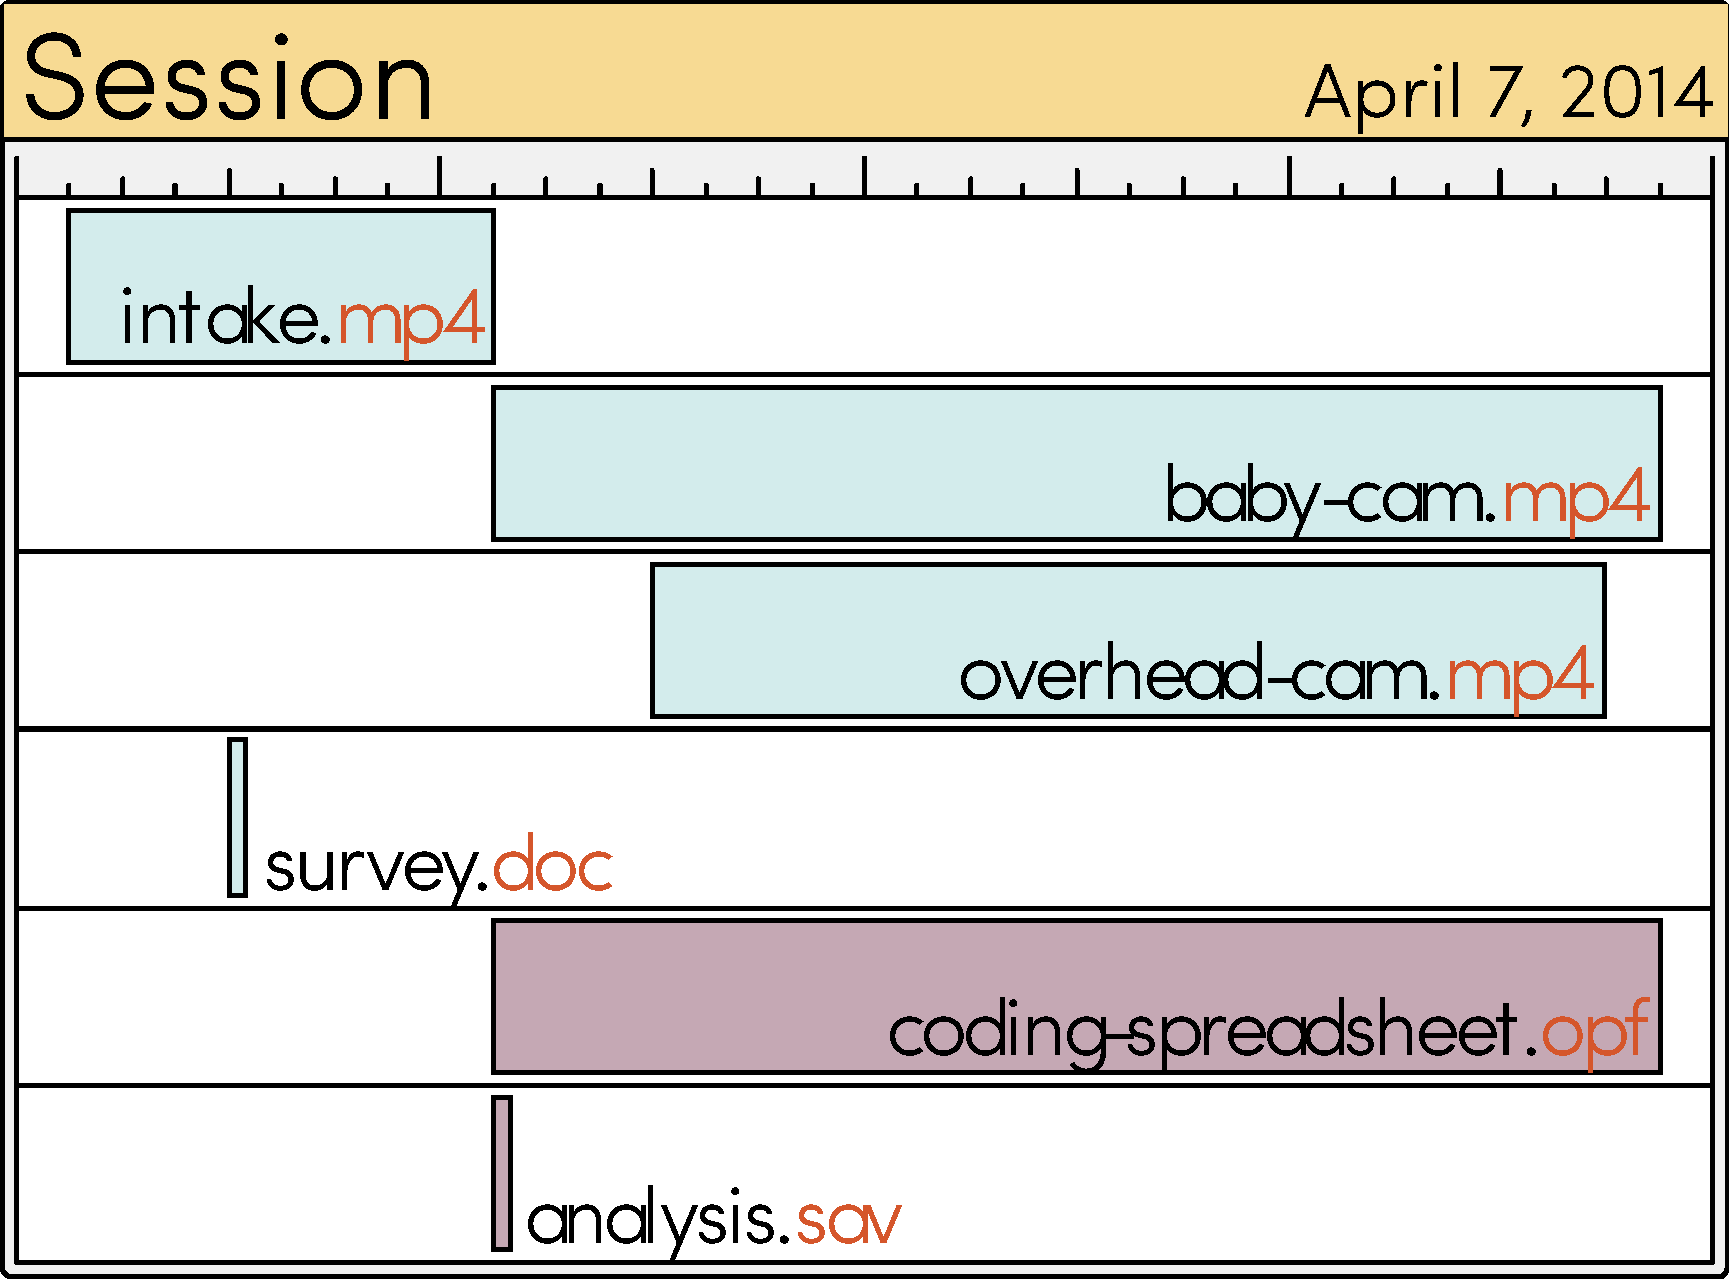
\includegraphics[width=\textwidth]{session.pdf}

	\column{\textwidth-2.25in}
	\begin{itemize}
		\item Covered by a \emph{release level}
		\item Data collected at the same time
		\item Contains timeline of collected raw data files
		\item Annotated with metadata
		\item Analysis files layered on
	\end{itemize}

	\end{columns}
\end{frame}

\begin{frame}{Datasets and Studies}{Data provenance}
	\begin{columns}
	\column{\textwidth-2.95in}
	\begin{itemize}
	\item Datasets: raw data collected directly during a session
	\item Studies: analyses, generated data, published papers
	\end{itemize}

	\column{2.5in}
	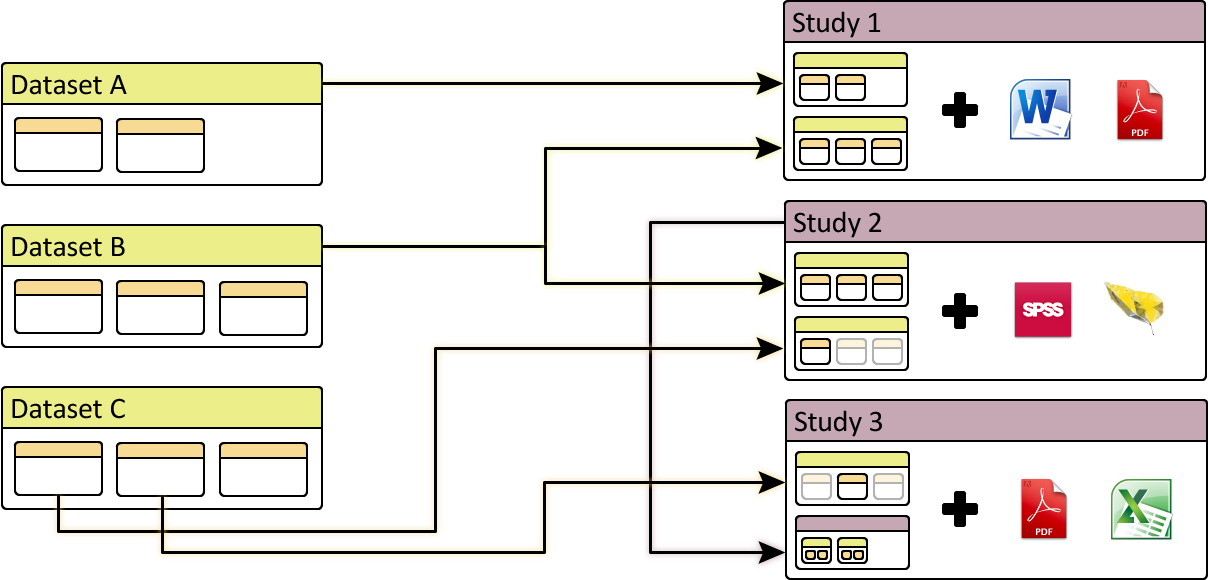
\includegraphics[width=2.5in]{studies.png}
	\end{columns}

	\begin{itemize}
	\item Studies collect included sessions from datasets and ``layer'' files over them
	\item Allows re-purposing, re-collecting data
	\end{itemize}
\end{frame}

\section{Walkthrough}

\begin{frame}{Walkthrough}{Live site}
\end{frame}

\section{Next steps}
\begin{frame}<1>[label=browser]{Next steps}{Enhancing the browser}
	\begin{itemize}
		\item<1> Improve searching, filtering, sorting within and across datasets
		\item<1> Have many user stores and use cases to drive this
		\item<2> Mainly focused around browsing, searching, using
		\item<2> Also want to build views that make sense for entering data, and can be reused for editing
	\end{itemize}
\end{frame}

\begin{frame}{User stories}{Education and Teaching}
	\begin{itemize}
		\item Video clips for teaching
		\item Illustrate an idea
		\item Show the range of behaviors and exceptions
		\item Show an excerpt in a talk
	\end{itemize}
\end{frame}
\begin{frame}{User stories}{Pre-research}
	\begin{itemize}
		\item Browse the work in my field
		\item Decide whether a study is worth doing
		\item Preliminary data for grant proposal
		\item Ideas and inspiration
		\item Replicate, expand on, or review previous work based on the procedure or coding manual
	\end{itemize}
\end{frame}
\begin{frame}{User stories}{Research}
	\begin{itemize}
		\item Repurpose videos for new uses
		\item Replicate existing work by recoding videos
		\item Grow sample size
		\item Include participants from other contexts and populations
		\item Conduct integrative analyses
		\item Complete a grant progress report
	\end{itemize}
\end{frame}
\againframe<2>{browser}

\begin{frame}{Databrary 1.0}{Public release}
	\begin{itemize}
		\item Better video, timeline management
		\item Improved browsing within a dataset/study
		\item Uploading as you go
		\item Entering, editing data
		\item Organizing, grouping data
	\end{itemize}
\end{frame}

\end{document}
